\subsubsection{Simulação de geração de energia}
\noindent A simulação de produção de energia solar foi realizada por meio da ferramenta PVsyst, versão v6.8.1 \cite{Cronemberger2012}. Esta ferramenta foi utilizada por disponibilizar a análise de desempenho e dimensionamento do sistema de produção de energia solar necessário para empreendimentos do porte da edificação proposta nesta pesquisa. Complementarmente a ferramenta, foi feito um levantamento dos módulos fotovoltaicos comercializados no Brasil de acordo com a aplicação destes componentes sobre a envoltória, como módulos monocristalinos de silício, m-Si, e filme fino de Telúrio de Cádmio, Cd-Te \cite{Didone2014,Werneck2017,Sorgato2018}. Estas tecnologias foram escolhidas por serem indicadas para a aplicação sobre as superfícies horizontais, como a cobertura e o estacionamento, e verticais, como as fachadas.\newline
\begin{table}[H]
    \small
    \caption{Módulos fotovoltaicos utilizados e a áreadisponível para implantação.}
    \begin{tabular}{lllll}
    \hline
    \multicolumn{2}{c}{\multirow{2}{*}{\textbf{Características}}}                                                                                   & \multicolumn{3}{c}{\textbf{Modelo genérico de 8 pavimentos}}                                                                                                                   \\ \cline{3-5} 
    \multicolumn{2}{c}{}                                                                                                                            & \multicolumn{1}{c}{\makecell[c]{\textbf{Cobertura} \\\textbf{e estacionamento}}}   & \multicolumn{1}{c}{\makecell[c]{\textbf{Proteção} \\ \textbf{solar}}}            & \multicolumn{1}{c}{\textbf{Fachada}}                      \\ \hline
    \multicolumn{1}{c}{\parbox[t]{2mm}{\multirow{8}{*}{\rotatebox[origin=c]{90}{\textbf{Módulo}}}}} & Módulo                                        & \multicolumn{1}{c}{\makecell[c]{SunPower \\SPR-E20-435-COM}}              & \multicolumn{1}{c}{\makecell[c]{SunPower \\SPR-E20-435-COM}}           & \multicolumn{1}{c}{\makecell[c]{First Solar \\FS-4122-2}}                 \\
    \multicolumn{1}{c}{}                                                                            & Tecnologia                                    & \multicolumn{1}{c}{m-SI}                                  & \multicolumn{1}{c}{m-SI}                               & \multicolumn{1}{c}{Cd-Te}                                 \\
    \multicolumn{1}{c}{}                                                                            & Potência máx. (Wp)                            & \multicolumn{1}{c}{435}                                   & \multicolumn{1}{c}{435}                                & \multicolumn{1}{c}{122,5}                                 \\
    \multicolumn{1}{c}{}                                                                            & Tensão máx. (V)                               & \multicolumn{1}{c}{324}                                   & \multicolumn{1}{c}{648}                                & \multicolumn{1}{c}{376}                                   \\
    \multicolumn{1}{c}{}                                                                            & \makecell[l]{Potência Nominal \\- STC (kWp)}  & \multicolumn{1}{c}{150}                                   & \multicolumn{1}{c}{100,92}                             & \multicolumn{1}{c}{274,22}                                \\
    \multicolumn{1}{c}{}                                                                            & Nº de módulos                                 & \multicolumn{1}{c}{345}                                   & \multicolumn{1}{c}{232}                                & \multicolumn{1}{c}{2238}                                  \\
    \multicolumn{1}{c}{}                                                                            & Eficiência (\%)                               & \multicolumn{1}{c}{19}                                    & \multicolumn{1}{c}{19}                                 & \multicolumn{1}{c}{17}                                    \\
    \multicolumn{1}{c}{}                                                                            & Área ocupada (m²)                             & \multicolumn{1}{c}{746}                                   & \multicolumn{1}{c}{501}                                & \multicolumn{1}{c}{1612}                                  \\ \hline
    \parbox[t]{2mm}{\multirow{5}{*}{\rotatebox[origin=c]{90}{\textbf{Inversor}}}}                   & Modelo                                        & \multicolumn{1}{c}{\makecell[c]{Fronius \\International \\IG Plus 150 V-3}} & \multicolumn{1}{c}{\makecell[c]{Fronius \\International \\ECO 25.0-3-S}} & \multicolumn{1}{c}{\makecell[c]{Fronius International \\IG Plus 150 V-3}} \\
                                                                                                    & Nº de inversores                              & \multicolumn{1}{c}{10}                                    & \multicolumn{1}{c}{6}                                  & \multicolumn{1}{c}{14}                                    \\
                                                                                                    & \makecell[l]{Potência máx. \\total (kWac)}    & \multicolumn{1}{c}{120}                                   & \multicolumn{1}{c}{50}                                 & \multicolumn{1}{c}{84}                                    \\
                                                                                                    & Tensão de entrada (V)                         & \multicolumn{1}{c}{230-500}                               & \multicolumn{1}{c}{580-850}                            & \multicolumn{1}{c}{230-500}                               \\
                                                                                                    & Eficiência (\%)                               & \multicolumn{1}{c}{97,9}                                  & \multicolumn{1}{c}{97,9}                               & \multicolumn{1}{c}{97,9}                                  \\ \hline
    \multicolumn{2}{c}{\multirow{2}{*}{\textbf{Características}}}                                   & \multicolumn{3}{c}{\textbf{Modelo genérico de 19 pavimentos}}                                                                                                                   \\ \cline{3-5} 
    \multicolumn{2}{c}{}                                                                            & \multicolumn{1}{c}{\makecell[c]{\textbf{Cobertura} \\\textbf{e estacionamento}}}                          & \multicolumn{1}{c}{\makecell[c]{\textbf{Proteção} \\ \textbf{solar}}}            & \multicolumn{1}{c}{\textbf{Fachada}}                      \\ \hline
    \multicolumn{1}{c}{\parbox[t]{2mm}{\multirow{8}{*}{\rotatebox[origin=c]{90}{\textbf{Módulo}}}}} & Módulo                                        & \multicolumn{1}{c}{\makecell[c]{SunPower \\SPR-E20-435-COM}}              & \multicolumn{1}{c}{\makecell[c]{SunPower \\SPR-E20-435-COM}}           & \multicolumn{1}{c}{\makecell[c]{First Solar \\FS-4122-2}}                 \\
    \multicolumn{1}{c}{}                                                                            & Tecnologia                                    & \multicolumn{1}{c}{Si-mono}                                  & \multicolumn{1}{c}{Si-mono}                               & \multicolumn{1}{c}{Cd-Te}                                 \\
    \multicolumn{1}{c}{}                                                                            & Potência máx. (Wp)                            & \multicolumn{1}{c}{435}                                   & \multicolumn{1}{c}{435}                                & \multicolumn{1}{c}{122,5}                                 \\
    \multicolumn{1}{c}{}                                                                            & Tensão máx. (V)                               & \multicolumn{1}{c}{324}                                   & \multicolumn{1}{c}{648}                                & \multicolumn{1}{c}{376}                                   \\
    \multicolumn{1}{c}{}                                                                            & \makecell[l]{Potência Nominal \\- STC (kWp)}  & \multicolumn{1}{c}{150}                                   & \multicolumn{1}{c}{243,40}                             & \multicolumn{1}{c}{479,70}                                \\
    \multicolumn{1}{c}{}                                                                            & Nº de módulos                                 & \multicolumn{1}{c}{345}                                   & \multicolumn{1}{c}{560}                                & \multicolumn{1}{c}{3917}                                  \\
    \multicolumn{1}{c}{}                                                                            & Eficiência (\%)                               & \multicolumn{1}{c}{19}                                    & \multicolumn{1}{c}{19}                                 & \multicolumn{1}{c}{17}                                    \\
    \multicolumn{1}{c}{}                                                                            & Área ocupada (m²)                             & \multicolumn{1}{c}{746}                                   & \multicolumn{1}{c}{745}                                & \multicolumn{1}{c}{2820}                                  \\ \hline
    \parbox[t]{2mm}{\multirow{5}{*}{\rotatebox[origin=c]{90}{\textbf{Inversor}}}}                   & Modelo                                        & \multicolumn{1}{c}{\makecell[c]{Fronius \\International \\IG Plus 150 V-3}} & \multicolumn{1}{c}{\makecell[c]{Fronius \\International \\ECO 25.0-3-S}} & \multicolumn{1}{c}{\makecell[c]{Fronius \\International \\IG Plus 150 V-3}} \\
                                                                                                    & Nº de inversores                              & \multicolumn{1}{c}{10}                                    & \multicolumn{1}{c}{13}                                  & \multicolumn{1}{c}{22}                                    \\
                                                                                                    & \makecell[l]{Potência máx. \\total (kWac)}    & \multicolumn{1}{c}{162}                                   & \multicolumn{1}{c}{125}                                 & \multicolumn{1}{c}{250}                                    \\
                                                                                                    & Tensão de entrada (V)                         & \multicolumn{1}{c}{580-850}                               & \multicolumn{1}{c}{580-850}                            & \multicolumn{1}{c}{580-850}                               \\
                                                                                                    & Eficiência (\%)                               & \multicolumn{1}{c}{97,9}                                  & \multicolumn{1}{c}{97,9}                               & \multicolumn{1}{c}{97,7}                                  \\ \hline
                                                                                                    &                                               &                                                           &                                                        &                                                          
    \end{tabular}
    \begin{flushleft}
        \par \small Fonte: autor, (2019).
    \end{flushleft}
    \label{tab:tabela14}
    \end{table}
    \vspace{-0.60cm} \noindent Foram simulados cenários de acordo com a aplicação da proteção solar proposta assim como para cada PAF\textsubscript{T}. Todavia, com a dimensão dos equipamentos de proteção solar definida, de acordo com a Tabela 14, foi levantada a quantidade de área disponível para a implantação dos módulos fotovoltaicos, segundo a incidência de irradiação solar sobre a superfície dos modelos e da latitude de Vitória.\newline
    \noindent Foi considerado 70\% da área do segundo pavimento de estacionamento para a instalação da estrutura de suporte aos módulos fotovoltaicos. Esta estrutura desempenharia a função de cobertura para os veículos, uma vez que esta área é descoberta e apresenta áreas de manobra e acesso as vagas. Além disso, a inclinação dos módulos foi configurada da seguinte forma:
    \begin{itemize}
        \item A área da cobertura e estacionamento com inclinação de 20°;
        \item Os módulos da fachada com 90° por estarem instalados nas superfícies opacas da fachada, perpendiculares ao piso; e
        \item Os módulos instalados nas proteções solares com inclinação de 5°, a fim de aumentar a incidência solar sobre os módulos sem comprometer a fachada, dificultar o deposito de sedimentos e facilitar a manutenção do sistema.
    \end{itemize}
    \noindent Para atingir a máxima produção de energia solar fotovoltaica, foi proposto o deslocamento das torres dos modelos para maior exposição da área de estacionamento à radiação solar, como exemplificado na Figura \ref{fig:figure22}. Vale lembrar que Plano Diretor vigente sobre o recorte territorial não limita a cobertura da área de cobertura do estacionamento em relação aos lotes circundantes, uma vez que a área em questão não está ao nível do térreo, permitindo a implementação das coberturas com painéis fotovoltaicos.\vspace*{-0.2cm}
    \begin{figure}[H]
        \caption{Deslocamento de torres dos modelos genéricos sobre as áreas de estacionamento. O volume tracejado demonstra a posição original da torre antes do deslocamento.}
        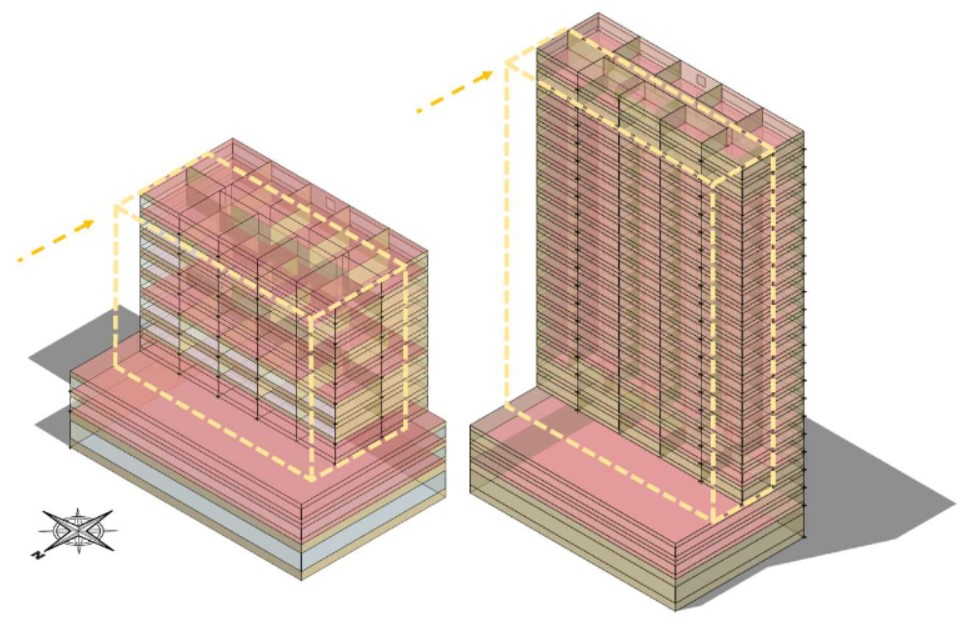
\includegraphics[width=1.0\textwidth]{figures/fig22-modelos.jpg}
        \begin{flushleft}
            \par \small Fonte: autor, (2019).
        \end{flushleft}
        \label{fig:figure22}
    \end{figure}